\chapter{Runoff generation} \label{chap:runGen}
\renewcommand{\tabdir}{chapters/part_processes/runoffGeneration/tab}
\renewcommand{\figdir}{chapters/part_processes/runoffGeneration/fig}

\section{Introduction} \label{sec:runGen_intro}

To avoid confusion, it is important to distinguish between the terms \emph{runoff generation} and \emph{runoff concentration}. As \emph{runoff generation}, we understand the transformation of water input (rain, snow melt) into runoff \emph{at the local scale}, \ie{} at every single point of a catchment. In contrast to that, the term \emph{runoff concentration} describes the transport of the locally generated runoff to the catchment's outlet (or the nearest river).

In some cases, the strict separation of the two terms is really pragmatic. However, it provides a clear and quite useful concept for hydrological catchment modeling.



%%%%%%%%%%%%%%%%%%%%%%%%%%%%%%%%%%%%%%%%%%%%%%%%%%%%%%%%%%%%%%%%%%%%%%%%%%%%%%%%
%%%%%%%%%%%%%%%%%%%%%%%%%%%%%%%%%%%%%%%%%%%%%%%%%%%%%%%%%%%%%%%%%%%%%%%%%%%%%%%%
%%%%%%%%%%%%%%%%%%%%%%%%%%%%%%%%%%%%%%%%%%%%%%%%%%%%%%%%%%%%%%%%%%%%%%%%%%%%%%%%
%%%%%%%%%%%%%%%%%%%%%%%%%%%%%%%%%%%%%%%%%%%%%%%%%%%%%%%%%%%%%%%%%%%%%%%%%%%%%%%%
%%%%%%%%%%%%%%%%%%%%%%%%%%%%%%%%%%%%%%%%%%%%%%%%%%%%%%%%%%%%%%%%%%%%%%%%%%%%%%%%




\section{Simple four components model} \label{sec:runGen4comp}

%%%%%%%%%%%%%%%%%%%%%%%%%%%%%%%%%%%%%%%%%%%%%%%%%%%%%%%%%%%%%%%%%%%%%%%%%%%%%%%%

\subsection{Processes and equations} \label{sec:runGen4comp_processes}

The four components runoff generation model described here is based on the concepts used in the LARSIM\footnote{Model variant '4Q-KOMP mit A2'} model \citet{Ludwig2006}. Originally, most equations were first presented by \citet{Todini1996}.

The runoff generation model is built upon the water balance of a soil column (\figref{fig:runGen4comp_soilWater}) which can be expressed by \eqnref{eqn:runGen4comp_soilWaterBalance}

\begin{equation} \label{eqn:runGen4comp_soilWaterBalance}
  \frac{d\soilWaterContent}{dt} = \frac{\rateWaterSupply - \rateRunoffSurf - \rateRunoffPref - \rateRunoffInter - \rateRunoffBase - \rateEvapotransp}{\soilDepth}
\end{equation}

with

\begin{tabular}{llp{0.6\columnwidth}}
\soilWaterContent & (--) & Soil water content as \cbm/\cbm \\
\rateWaterSupply & (m/s) & Rate of water supply (see \eqnref{eqn:runGen4comp_waterSupply}) \\
\rateRunoffSurf & (m/s) & Rate of surface runoff \\
\rateRunoffPref & (m/s) & Rate of quick sub-surface runoff (preferential flow) \\
\rateRunoffInter & (m/s) & Rate of slow sub-surface runoff (interflow) \\
\rateRunoffBase & (m/s) & Rate of deep percolation (rate of ground water recharge) \\
\rateEvapotransp & (m/s) & Rate of evapo(transpi)ration \\
\soilDepth & (m) & Depth (thickness) of soil column. \\
\end{tabular}

\medskip
The relevant thickness of the soil column \soilDepth{} is equivalent to the rooted depth. Soil water at greater depths is assumed (1) to be unavailable for evapotranspiration and (2) not to contribute to lateral runoff processes.

\begin{figure}
  \includegraphics[width=0.9\columnwidth]{\figdir/soilWaterFluxes.eps}
  \caption{Water fluxes with respect to a soil column with (right) and without snow cover (left). \label{fig:runGen4comp_soilWater}}
\end{figure}

Snow coverage of the soil column is assumed to be either 0 or 100\%, \ie{} partial covering is \emph{not} simulated. As long as no snow is present, the rate of water supply to the soil column is the same as the intensity of precipitation, \precipIntensity{}. Once a snow cover exists, all precipitation is trapped in the snow and the rate of water supply is controlled by the melt rate, \rateSnowMelt{} (\eqnref{eqn:runGen4comp_waterSupply}). Both \precipIntensity{} and \rateSnowMelt{} are in units of m/s.

\begin{align} \label{eqn:runGen4comp_waterSupply}
  \rateWaterSupply =
  \begin{cases}
    \rateSnowMelt & \text{if snow cover is present} \\
    \precipIntensity & \text{else} \\
  \end{cases}
\end{align}

In the presented four components model, the generation of direct runoff\footnote{Runoff being quickly generated in response to water input.} is bound to the existence of (local) soil saturation. Thus, the model accounts for surface runoff due to infiltration excess but \emph{not} for Hortonian surface runoff.

Following to the Xinanjiang approach \citep{Zhao1980}, the fraction of saturated areas \satFrac{} in a catchment can be estimated from the area-integrated relative saturation of the soil \relSat{} which is the ratio of the current and maximum soil water content \soilWaterContent{} and \soilWaterContentMax{}, respectively (\eqnsref{eqn:runGen4comp_relativeSaturation} and \ref{eqn:runGen4comp_satFrac}). The rationale of the Xinanjiang model is a positive correlation between the catchment's average wetness, represented by the relative filling of the soil reservoir and the proportion of saturated areas. In other words, the occurrence of local saturation is assumed to increases as the catchment's average wetness becomes higher.

\begin{align}
  \relSat =& \frac{\soilWaterContent}{\soilWaterContentMax} \label{eqn:runGen4comp_relativeSaturation} \\
  \satFrac=& 1 - \left( 1 - \relSat \right) ^ \expSatFrac \label{eqn:runGen4comp_satFrac}
\end{align}

The shape of the relation between \relSat{} and \satFrac{} is controlled by a dimensionless empirical parameter \expSatFrac{}. The effect of different values of \expSatFrac{} is illustrated in \figref{fig:runGen4comp_expSatFrac}. A linear relation is assumed in the case $\expSatFrac{}=1$. Note that only values of $\expSatFrac{} \le 1$ are physically reasonable.

\begin{figure}
  \includegraphics[width=0.9\columnwidth,angle=270]{\figdir/xinanjiang.eps}
  \caption[Influence of the empirical parameter \expSatFrac{}.]{Influence of the empirical parameter \expSatFrac{} on the relation between the catchment-integrated relative filling of the soil reservoir (x-axis) and the fraction of saturated areas \satFrac{} (y-axis). Only values of $\expSatFrac{} \le 1$ are physically reasonable. \label{fig:runGen4comp_expSatFrac}}
\end{figure}

The amount of direct runoff \heightRunoffDirect{} (in meters) is computed as a function of the fraction of saturated areas \satFrac{} according to \eqnref{eqn:runGen4comp_surfaceDirect}

\begin{align*}
  \heightRunoffDirect=
  \begin{cases}
    I - (W_m - W) + W_m \cdot x^{\expSatFrac+1}  & if (x > 0) \\
    I - (W_m - W)) & if (x \le 0)
  \end{cases}
\end{align*}

with

\begin{align} \label{eqn:runGen4comp_surfaceDirect}
  x=& \left(1-\frac{W}{W_m}\right)^{\left(\frac{1}{\expSatFrac+1}\right)} - \frac{I}{(1+\expSatFrac) \cdot W_m}
\end{align}

and $I$ being the total water input in a time step ($I= \rateWaterSupply \cdot \deltat$), $W$ being the amount of water in the modeled soil column ($W= \soilWaterContent \cdot \soilDepth$) and $W_m$ being the maximum capacity of the soil column ($W_m= \soilWaterContentMax \cdot \soilDepth$), all in units of meters. The derivation of this expression can be found in \citet{Todini1996} but is has to be noted that in this publication some signs are incorrect. The corrected version is presented in \citet{Bremicker2006}, for example. The relation between \heightRunoffDirect{} and $I$ according to \eqnref{eqn:runGen4comp_surfaceDirect} is illustrated in \figref{fig:runGen4comp_directRunoffHeight} for fix values of $W$ and $W_m$. A retention effect is visible for small to moderate water inputs. For water inputs considerably higher than the initial storage capacity of the soil, the relation between \heightRunoffDirect{} and $I$ becomes linear.

\begin{figure}
  \includegraphics[width=0.9\columnwidth,angle=270]{\figdir/arno.eps}
  \caption{Direct runoff computed with \eqnref{eqn:runGen4comp_surfaceDirect} for example values of soil storage and water input. \label{fig:runGen4comp_directRunoffHeight}}
\end{figure}

The model described here distinguished two components of direct runoff which differ with respect to retention characteristics. They may be considered as surface runoff and quick subsurface runoff through preferential flow paths. The proportion of the two components is controlled by a threshold value \thresholdSurf{} in units of m/s. The rates of surface runoff and quick subsurface runoff are computed according to \eqnref{eqn:runGen4comp_surfaceRunoff} and \eqnref{eqn:runGen4comp_prefRunoff}

\begin{align}
  \rateRunoffSurf =& max\left( 0, \frac{\heightRunoffDirect}{\deltat} - \thresholdSurf \right) \label{eqn:runGen4comp_surfaceRunoff} \\
  \rateRunoffPref =& \frac{\heightRunoffDirect}{\deltat} - \rateRunoffSurf \label{eqn:runGen4comp_prefRunoff}
\end{align}

Thus, if the rate of direct runoff production $\heightRunoffDirect/\deltat$ is below the threshold \thresholdSurf{}, only subsurface runoff is generated. Otherwise, surface runoff is generated from the excessive water. Note that the settings $\thresholdSurf{}=0$ or $\thresholdSurf{} \rightarrow \infty$ effectively result in a model with only 3 runoff components.

The generation of the slow runoff components is closely linked to the relative saturation of the soil \relSat{} (\eqnref{eqn:runGen4comp_relativeSaturation}). The rate of interflow runoff is computed by \eqnref{eqn:runGen4comp_interRunoff} using three empirical parameters. Here, \facInter{} represents a maximum rate of interflow runoff generation corresponding to total saturation of the soil. The actual rate, \rateRunoffInter{}, decreases at lower values of the soil saturation. If the saturation falls below a threshold level \relSatInter{}, no interflow runoff is generated at all. The shape of the soil moisture dependence is controlled by the empirical exponent \expInter{} whose effect is illustrated in \figref{fig:runGen4comp_powerExpression} (argument $s$ represents the fractional expression of \eqnref{eqn:runGen4comp_interRunoff}). The higher the value of the empirical exponent, the wetter the soil needs to be for interflow runoff becoming an important component. At very low values of \expInter{}, interflow runoff is produced almost at the maximum rate \facInter{}, as soon as the soil saturation exceeds the threshold \relSatInter{}. As in LARSIM, the parameter \expInter{} is treated as a constants with a value of 1.5 \citep{Bremicker2006}.

\begin{align} \label{eqn:runGen4comp_interRunoff}
  \rateRunoffInter =
  \begin{cases}
    \facInter \cdot \left( \frac{\relSat-\relSatInter}{1 - \relSatInter} \right) ^ \expInter & \text{if} \; \relSat > \relSatInter \\
    0 & \text{if} \; \relSat \le \relSatInter \\
  \end{cases}
\end{align}

\begin{figure}
  \includegraphics[width=0.9\columnwidth,angle=270]{\figdir/powerExpression.eps}
  \caption{Effect of the exponent $E$ in a formula $f=s^E$ for $s$ in range [0,1]. \label{fig:runGen4comp_powerExpression}}
\end{figure}

The rate of groundwater recharge (or base flow runoff), \rateRunoffBase{}, is computed by \eqnref{eqn:runGen4comp_baseRunoff} which is conceptually identical to \eqnref{eqn:runGen4comp_interRunoff}. Here, \facBase{} is the maximum rate of groundwater recharge which corresponds to a saturated soil. If the relative saturation of the soil falls below \relSatBase{}, the rate of groundwater recharge becomes zero. The shape of the dependence between \rateRunoffBase{} and \relSat{} is controlled by the empirical exponent \expBase{}. Again, the effect of this exponent can be seen from \figref{fig:runGen4comp_powerExpression} (argument $s$ represents the fractional expression of \eqnref{eqn:runGen4comp_baseRunoff}). As in LARSIM, the parameters \relSatBase{} and \expBase{} are treated as a constants with values of 0.05 and 1, respectively \citep{Bremicker2006}. Thus, only \facBase remains as a calibration parameter.

\begin{align} \label{eqn:runGen4comp_baseRunoff}
  \rateRunoffBase=
  \begin{cases}
    \facBase \cdot \left( \frac{\relSat-\relSatBase}{1 - \relSatBase} \right) ^ \expBase & \text{if} \; \relSat > \relSatBase \\
    0 & \text{if} \; \relSat \le \relSatBase \\
  \end{cases}
\end{align}

Of course, the theory described so far is only applicable to areas where soil water storage occurs. For areas covered by water or impervious surfaces, the rate of surface runoff \rateRunoffSurf{} equals the rate of rainfall or snow melt, respectively.

%%%%%%%%%%%%%%%%%%%%%%%%%%%%%%%%%%%%%%%%%%%%%%%%%%%%%%%%%%%%%%%%%%%%%%%%%%%%%%%%

\subsection{Combination with other models} \label{sec:runGen4comp_combination}
Depending on the model's purpose and local conditions, the described runoff generation model has to be augmented with
\begin{itemize}
  \item a model to compute snow storage and melt,
  \item a model to estimate evapotranspiration,
  \item an approach for precipitation correction (if not done externally).
\end{itemize}

%%%%%%%%%%%%%%%%%%%%%%%%%%%%%%%%%%%%%%%%%%%%%%%%%%%%%%%%%%%%%%%%%%%%%%%%%%%%%%%%

\subsection{Mathematical solution} \label{sec:runGen4comp_solution}

\eqnref{eqn:runGen4comp_soilWaterBalance} is an ordinary differential equation. Depending on the use of the model, a more of less sophisticated numerical solution has to be adopted. If computation times are critical (\eg{} in operational models), a simple \first{} order numerical solution may be preferable. Then, however, it needs special efforts to prevent unstable or unphysical solutions. In particular, in the absence of appropriate correction terms, a \first{} oder solution of \eqnref{eqn:runGen4comp_soilWaterBalance} may yield a computed soil moisture \soilWaterContent{} which is negative.

%%%%%%%%%%%%%%%%%%%%%%%%%%%%%%%%%%%%%%%%%%%%%%%%%%%%%%%%%%%%%%%%%%%%%%%%%%%%%%%%

\subsection{Implementation} \label{sec:runGen4comp_implementation}

\tabref{tab:runGen4comp_implementation} relates the identifier names used in the model implementation (names of state variables and parameters) to the symbols used in the process equations (\secref{sec:runGen4comp_processes}). Additional information that may be helpful when calibrating a model without any prior knowledge of parameter values is given in \secref{sec:runGen4comp_hints}.

\begin{table*}
\caption{Symbols used in the process equations (\secref{sec:runGen4comp_processes}), corresponding identifiers, and hints for calibration. \label{tab:runGen4comp_implementation}}
\begin{tabular}{|p{0.07\textwidth}p{0.15\textwidth}p{0.1\textwidth}p{0.15\textwidth}p{0.35\textwidth}|}  \hline
\rowcolor[gray]{0.9}
Symbol & Identifier & Units & Typical values & Details \\ \hline
\soilWaterContent & \verb!wc! & -- & -- & Computed state variable \\
\soilDepth & \verb!soildepth! & m & Rooted depth & -- \\
\soilWaterContentMax & \verb!wc_max! & -- & 0.4--0.5 & \tabref{tab:eta:soilmoisture} on page \pageref{tab:eta:soilmoisture} \\
\expSatFrac & \verb!exp_satfrac! & -- & 0.01--1 & See \figref{fig:runGen4comp_expSatFrac} \\
\thresholdSurf & \verb!thr_surf! & m/s & --  & Values of 0 or near $\infty$ result in a 3 components model (see \eqnsref{eqn:runGen4comp_surfaceRunoff} \& \ref{eqn:runGen4comp_prefRunoff} ). \\
\relSatInter & \verb!relsat_inter! & -- & 0.5 -- 0.8 & Number between 0 and 1. \\
\rateRunoffInter & \verb!rate_inter! & m/s & example: 1.e-07 & Depends on hydraulic conductivity \\
\rateRunoffBase & \verb!rate_base! & m/s & example: 1.e-08 & Depends on hydraulic conductivity \\
\hline
\end{tabular}
\end{table*}

\subsection{Hints for application} \label{sec:runGen4comp_hints}

The parameter \facBase{} specifies the rate of deep percolation under the conditions of a fully saturated soil (\eqnref{eqn:runGen4comp_baseRunoff}). At a first glance, it seems as if \facBase{} could be estimated from the soil's saturated hydraulic conductivity \satHydrCond{}. However, at high values of the soil moisture, the other runoff components are also active and, typically, these other components are much more effective in draining the soil. Consequenty, we can expect \facBase{} $\ll$ \satHydrCond{}.

A more promising approach to estimate \facBase{} relies on the analysis of a discharge hydrograph (\figref{fig:runGen4comp_parEstim_facBase}). In this figure, an approxiate hydrograph of the base flow component was added. It can be drawn by hand as a smooth line connecting the annual minimum values (low flows) also touching the minima during the rainy season. Obviously, the hydrograph of the base flow component has, like any periodic function, two types of turning points. For convenience, we focus on the lower turning points here. They are easier to identify from the data without the need for any drawing, actually.

\begin{figure}
  \includegraphics[width=0.9\columnwidth]{\figdir/parEstim_facBase.eps}
  \caption{Discharge hydrograph with manually separated base flow component. \label{fig:runGen4comp_parEstim_facBase}}
\end{figure}

In the following we assume that the base flow component is equivalent to the outflow from a conceptual ground water reservoir. For simplicity, we may consider a linear reservoir described by \eqnsref{eqn:runConcParStor_linResBalance} \& \ref{eqn:runConcParStor_linResOutflow} (see page \pageref{eqn:runConcParStor_linResBalance}). From the differential equation, we find that, at the mentioned turning points, the derivative of the storage volume with respect to time becomes zero, hence the rates of inflow and outflow are equal. Consequently, the \emph{base flow rate} at the turning points in a plot like \figref{fig:runGen4comp_parEstim_facBase} directly yields an estimate of the \emph{rate of ground water recharge}, \rateRunoffBase{}, at the respective point in time.

The relation between the actual rate of ground water reacharge \rateRunoffBase{} and the model parameter \facBase{} is given by \eqnref{eqn:runGen4comp_baseRunoff}. This can be rearranged and \rateRunoffBase{} can be substituted by $A \cdot Q_{base}$ where $A$ is the size of the catchment in units of \sqm{} and $Q_{base}$ is the base flow component in \cbms{} (\eqnref{eqn:runGen4comp_parEstim_facBase}). Using the fixed values of \relSatBase{} and \expBase{} mentioned in  \secref{sec:runGen4comp_processes}, we end up with \eqnref{eqn:runGen4comp_parEstim_facBase_final}.

\begin{eqnarray}
  \facBase &=& \dfrac{Q_{base}}{A} \cdot \left( \dfrac{\relSat-\relSatBase}{1 - \relSatBase} \right) ^ {-\expBase} \label{eqn:runGen4comp_parEstim_facBase} \\
           &=& \dfrac{Q_{base}}{A} \cdot \left( \dfrac{0.95}{\relSat - 0.05} \right) \label{eqn:runGen4comp_parEstim_facBase_final}
\end{eqnarray}

In order to calculate \facBase{} from \eqnref{eqn:runGen4comp_parEstim_facBase_final} we have to supply an estimate of the soil saturation \relSat{} at the respective point in time (\ie{} the analyzed turning point). For the lower turning points, a reasonable guess can be obtained from the soil water content at the wilting point. For a silty soil, for example, the saturation \relSat{} would be $\approx$ 0.2 for a soil moisture at the wilting point of 0.1 and a maximum water content of 0.48 (see \tabref{tab:eta:soilmoisture} on page~\pageref{tab:eta:soilmoisture}).

The value of \facBase{} obtained from the hydrograph analysis is a crude estimate. However, it might help in the definition of a proper search range for \facBase{} in the context of automatic model calibration.




%%%%%%%%%%%%%%%%%%%%%%%%%%%%%%%%%%%%%%%%%%%%%%%%%%%%%%%%%%%%%%%%%%%%%%%%%%%%%%%%
%%%%%%%%%%%%%%%%%%%%%%%%%%%%%%%%%%%%%%%%%%%%%%%%%%%%%%%%%%%%%%%%%%%%%%%%%%%%%%%%
%%%%%%%%%%%%%%%%%%%%%%%%%%%%%%%%%%%%%%%%%%%%%%%%%%%%%%%%%%%%%%%%%%%%%%%%%%%%%%%%
%%%%%%%%%%%%%%%%%%%%%%%%%%%%%%%%%%%%%%%%%%%%%%%%%%%%%%%%%%%%%%%%%%%%%%%%%%%%%%%%
%%%%%%%%%%%%%%%%%%%%%%%%%%%%%%%%%%%%%%%%%%%%%%%%%%%%%%%%%%%%%%%%%%%%%%%%%%%%%%%%




\section{Process-based approaches} \label{sec:rungen:proc}

In contrast to the simple conceptual four components model of \secref{sec:runGen4comp} the present section focuses on a process-based description of runoff generation. That means, each process of runoff generation, viz. infiltration into the soil, and vertical and horizontal soil water movement, shall be explicitly calculated. Together with evapotranspiration, interception, and snow storage and melt, which are described in independent chapters, this implicitly leads essentially to the same runoff components mentioned in \secref{sec:runGen4comp}. 

Note that the term \emph{process-based} refers to the explicit treatment of physical processes which are, however, often calculated using more or less empirical relationships as a detailed physical description is often not possible.



%%%%%%%%%%%%%%%%%%%%%%%%%%%%%%%%%%%%%%%%%%%%%%%%%%%%%%%%%%%%%%%%%%%%%%%%%%%%%%%%
%%%%%%%%%%%%%%%%%%%%%%%%%%%%%%%%%%%%%%%%%%%%%%%%%%%%%%%%%%%%%%%%%%%%%%%%%%%%%%%%


\subsection{Soil water movement}
In the following, ECHSE's process implementations of infiltration and soil water movement shall be described.


\subsubsection{Infiltration} \label{sec:rungen:inf}
Infiltration is the process of water uptake by the soil surface. The amount of water that can infiltrate is determined by the infiltration capacity of the soil which depends on soil texture properties and the current moisture state.

In the following the infiltration calculation approaches implemented in ECHSE are presented. They are accessible by calling the infiltration function and selecting the specific method via a choice parameter. The function's input is presented and shortly described in \tabref{tab:inf}. It returns the actual infiltration flux averaged over the simulation time step in [\si{\metre\per\second}]. The equations presented in the following refer to the infiltration capacity, i.e. the maximum possible infiltration flux $f_{max}$. The actual amount of infiltration $f_{act}$ is then derived by considering the incoming surface water flux for infiltration $R_f$:

\begin{equation}
f_{act} = min(R_f, f_{max})
\end{equation}

That means, the nonlinear infiltration process over the simulation time step is averaged to obtain a rate of volume change suitable for easy updating of the model's state variables defined in the respective model engine.\\

\noindent
Usage
\begin{verbatim}
infiltration(ch_inf,input,wc,wc_sat,
ksat,delta_t,na_val,
Hort_ini,Hort_end,Hort_k,
Phil_s,Phil_a,Phil_cal,
suc)
\end{verbatim}

\onecolumn
\begin{center}
\tablecaption{Argument list for ECHSE's master function \emph{infiltration} in the order of occurrence (check the source code for the case of unreported changes!).  \label{tab:inf}}
\tablefirsthead{}
\tablehead{
\multicolumn{5}{l}{\emph{Continued from previous page.}}\\ \hline
}
\tabletail{
\hline
\multicolumn{5}{l}{\emph{Continued on next page.}}\\
}
\tablelasttail{}
\begin{supertabular}{|p{0.06\textwidth}p{0.15\textwidth}p{0.05\textwidth}p{0.23\textwidth}p{0.36\textwidth}|} \hline
\rowcolor[gray]{0.9}
\hline
Symbol & Identifier & Unit & Explanation & Comment \\ \hline
\multicolumn{5}{|l|}{General input and parameters}\\ \hline
-- & \verb!ch_inf! & -- & Choice flag for infiltration method & 1: Horton's equation \newline 2: Philip's equation \newline 3: Green-Ampt two-stage model for layered soil \\
$R_f$ & \verb!input! & \si{\metre\per\second} & Surface water flux for infiltration & Typically precipitation, reduced by interception plus interception precipitation, plus snow melt plus lateral surface water inflow \\
\waterCont & \verb!wc! & \si{\cubic\metre\per\cubic\metre} & Actual volumetric water content of top soil & -- \\
\waterContSat & \verb!wc_sat! & \si{\cubic\metre\per\cubic\metre} & Volumetric water content at saturation of top soil & -- \\
\satHydrCond & \verb!ksat! & \si{\metre\per\second} & Saturated hydraulic conductivity & -- \\
\deltat & \verb!delta_t! & \si{\second} & Time step length & Temporal resolution of the model; \textbf{use ECHSE's internal parameter!} (only argument for the \verb!simulate! method, cf. \citet{Echse-Main-Doc}) \\
-- & \verb!na_val! & -- & Numeric value treated as \emph{not available (NA)} & Input quantities having the specified value will be internally treated as NA (e.g. for input checks) \\
\hline
\multicolumn{5}{|l|}{Horton's equation specific parameters}\\ \hline
$f_i$ & \verb!Hort_ini! & \si{\metre\per\second} & Initial infiltration rate & Parameter for Horton's equation; should be estimated from infiltration experiments or calibrated \\
$f_e$ & \verb!Hort_end! & \si{\metre\per\second} & Final infiltration rate & Parameter for Horton's equation; should be estimated from infiltration experiments or calibrated \\
$\beta$ & \verb!Hort_k! & \si{\metre\per\second} & Decay constant & Parameter for Horton's equation describing infiltration decay from $f_i$ to $f_e$ over time; should be estimated from infiltration experiments or calibrated \\
\hline
\multicolumn{5}{|l|}{Philip's equation specific parameters}\\ \hline
\sorptivity & \verb!Phil_s! & \si{\metre\per\second\tothe{1/2}} & Sorptivity & Parameter for Philip's equation; should be estimated from infiltration experiments or calculated from soil parameters, see \secref{sec:inf:philip} \\
$A$ & \verb!Phil_a! & \si{\metre\per\second} & Parameter & Parameter for Philip's equation; should be estimated from infiltration experiments or estimated from \satHydrCond{} and $k_A$, see \secref{sec:inf:philip} \\
$k_A$ & \verb!Phil_cal! & -- & Calibration parameter & Calibration parameter for Philip's equation; for estimation of $A$, in the range of [\num{0.2}..\num{1.0}], see \secref{sec:inf:philip} \\
\hline
\multicolumn{5}{|l|}{Green-Ampt specific parameters}\\ \hline
\capilSucWetfront & \verb!suc! & \si{\metre} & Capillary suction at the wetting front & Soil-specific parameter, can be derived by pedotransfer functions; \textbf{note} that unit [\si{\metre}] is approximately equal to \SI{100}{\hecto\pascal} \\
\hline
\end{supertabular}
\end{center}
\twocolumn


\paragraph{Horton's equation}
The infiltration model of Horton is a famous and simple empirical relationship and already applied for a long time \citep{Horton1933}. It is based on the observation that the infiltration capacity $f$ during an event exponentially declines since onset of the storm (time $t$) from an initial value $f_i$ approaching a constant value $f_e$ whereas the shape of the decline is defined by a shape parameter $\beta$ \citep{Horton1939}:

\begin{equation}
f = f_e + (f_i - f_e) e^{- \beta t}
\end{equation}

\noindent
Integration leads to the potentially cumulated infiltration:

\begin{equation}
F = f_e t + \frac{1}{\beta} (f_i - f_e) (1 - e^{- \beta t})
\end{equation}

The parameters are empirical and to be derived from infiltration experiments. However, for specific soil types values are reported in the literature that could be used (e.g. \citet{Maidment1993}).

\textbf{Note} that this equation should be applied to a single event whereas a typical application within ECHSE at discrete time steps would treat each call to the infiltration function as individual event. Soil moisture is not explicitly accounted for. You should therefore \textbf{not} use this approach in a typical continuous discrete time step application but apply it only to a single event! A further assumption is that incoming surface water flux for infiltration is at all times larger than the infiltration capacity. Recovery of infiltration capacity after an rainfall event is also not accounted for.


\paragraph{Philip's equation}\label{sec:inf:philip}
Philip's equation was directly derived from Richards equation (i.e. Darcy's law combined with the continuity equation) of flow through porous media. It was developed from the vertical description of flow assuming a homogeneous semi-infinite medium with constant initial soil moisture content and excess water available at the surface. The partial differential equation was approximated by a power series in $t^{1/2}$ whereas only the first two terms were considered as important and rearranged gave the simplified physically-based empirical equations for (potential) infiltration flux $f$ and the cumulated infiltration $F$ as \citep{Philip1957a,Philip1957d}:

\begin{equation}
f = \frac{1}{2} \sorptivity t^{-1/2} + A
\end{equation}

\noindent
and

\begin{equation}
F = \sorptivity t^{1/2} + A t
\end{equation}

\noindent
with\\ \vspace*{2ex}

\tablefirsthead{}
\tablehead{}
\tabletail{}
\tablelasttail{}
\begin{supertabular}{lp{0.75\columnwidth}}
  $t$ & Time since start of infiltration event (s) \\
  \sorptivity & Sorptivity, see text (\si{\metre\per\second\tothe{1/2}}) \\
  $A$ & Parameter proportional (but not equal to) saturated hydraulic conductivity, see text (\si{\metre\per\second}) \\
\end{supertabular}\\ \vspace*{2ex}

For small $t$ the first term of the equation is dominant, simulating horizontal water movement as function of $t^{1/2}$ and sorptivity. The latter was the most dominant quantity of the first term in the derivation of the equation where \citet{Philip1957d} interpreted the physical meaning as being \emph{"a measure of the capillary uptake or removal of water"}. As it hence embraces both adsorption and desorption the more general term \emph{sorptivity} was chosen for the parameter. It is a property of the medium, depending on soil texture and initial soil moisture content, and should be derived from experiments. However, there also exist some relations to soil properties. Currently implemented in ECHSE is an approach which already appeared in \citet{GreenAmpt1911} (though not under the term \emph{sorptivity} which was defined by \citet{Philip1957d}) as given by \citet{Stewart2013}:

\begin{equation}
\sorptivity = \sqrt{2 \satHydrCond (\waterContSat - \waterCont) \capilSucWetfront}
\end{equation}

\noindent
Usage
\begin{verbatim}
sorptivity(wc,wc_sat,ksat,suc)
\end{verbatim}

\noindent
with\\ \vspace*{2ex}

\tablefirsthead{}
\tablehead{}
\tabletail{}
\tablelasttail{}
\begin{supertabular}{lp{0.75\columnwidth}}
  \waterCont & Actual volumetric water content of top soil, \verb!wc! (\si{\cubic\metre\per\cubic\metre}) \\
  \waterContSat & Volumetric water content at saturation of top soil, \verb!wc_sat! (\si{\cubic\metre\per\cubic\metre}) \\
  \capilSucWetfront & Capillary suction at the wetting front; soil-specific parameter, can be derived by pedotransfer functions; \verb!suc! (\si{\metre}); \textbf{note} that unit is approximately equal to \SI{100}{\hecto\pascal} \\
  \satHydrCond & Saturated hydraulic conductivity, \verb!ksat! (\si{\metre\per\second}) \\
\end{supertabular}\\ \vspace*{2ex}

\noindent
This function is called internally if, when calling the \verb!infiltration! function, sorptivity (\verb!Phil_s!) was set to NA (\verb!na_val!). \citet{Stewart2013} also gives a better approximation of sorptivity which is, however, much more complicated and requires to solve an integral and was thus not yet implemented in ECHSE.

For growing $t$ the second term becomes more and more dominant as, when the soil becomes more saturated, gravitation is dominant over capillary pressure. It is clear that for $t\to\infty$ the infiltration rate approximates the saturated hydraulic conductivity \satHydrCond{}. Due to the power series approximation in the derivation of the equation, however, parameter $A$ can be related but is not equal to \satHydrCond{}. This also implies that the equation fails for large $t$ (in a test study in \citet{Philip1957d} the error for \SI{e6}{\second}, i.e. about \num{11.5} days, was \SI{5}{\percent}). Ideally, this parameter should as well be estimated from infiltration experiments. However, if the parameter (\verb!Phil_a!) is set to NA (\verb!na_val!) when calling \verb!infiltration! it is approximated from \satHydrCond{} (as, e.g., in \citet{Kreye2010en}):

\begin{equation}
A = \satHydrCond k_A
\end{equation}

\noindent
with $k_A$ being a parameter roughly in the the range of [\num{0.2}..\num{1.0}] that should be calibrated.


\paragraph{Green-Ampt two-stage approach for homogeneous layered soil}
The approach implemented in ECHSE is based on the approach used in the WASA \citep{Guentner2002} and WaSiM-ETH \citep{Schulla1997} models which build upon the semi-physical suction gradient-based method of \citet{GreenAmpt1911} and the extended two-stage model for layered soils. In the German language community this approach is often referred to \citet{Peschke1977,Peschke1987} whereas the oldest publications of this method I could so far (Feb. 2016) find are \citet{Mein1971,Mein1973}. See also common text books such as \citet{Dyck1995} or \citet{Chow1988} for an English version.

First the refillable porosity is calculated:

\begin{equation}
\porosRefill = \waterContSat - \waterCont
\end{equation}

\noindent
with\\ \vspace*{2ex}

\tablefirsthead{}
\tablehead{}
\tabletail{}
\tablelasttail{}
\begin{supertabular}{lp{0.75\columnwidth}}
  \porosRefill & Refillable porosity (--) \\
  \waterCont & Actual volumetric water content of top soil, \verb!wc! (\si{\cubic\metre\per\cubic\metre}) \\
  \waterContSat & Volumetric water content at saturation of top soil, \verb!wc_sat! (\si{\cubic\metre\per\cubic\metre}) \\
\end{supertabular}\\ \vspace*{2ex}

\noindent
and if the soil is saturated, i.e. if $\porosRefill = 0$, the function will return an infiltration rate equal to saturated hydraulic conductivity \satHydrCond{}. If the soil is not saturated and the incoming water flux is less than or equal to \satHydrCond{}, all the incoming water may infiltrate over the simulation time step and no saturated of the soil surface will occur. If the incoming water flux, however, is larger than \satHydrCond{} the approach implies a sharp wetting front evenly propagating through the soil. Initiation of infiltration is largely dominated by the matric potential. With successive wetting infiltration approaches \satHydrCond{} and the process is maintained by gravitation. The part above the wetting front is assumed to be at saturation whereas antecedent soil moisture is assumed for the soil below. The depth of the wetting front at the point of saturation of soil surface can be calculated using the following relation:

\begin{equation}
D_{wet} = \frac{\capilSucWetfront}{R_f / \satHydrCond - 1}
\end{equation}

\noindent
with\\ \vspace*{2ex}

\tablefirsthead{}
\tablehead{}
\tabletail{}
\tablelasttail{}
\begin{supertabular}{lp{0.75\columnwidth}}
  $D_{wet}$ & Depth of wetting front at saturation (\si{\metre}) \\
  \capilSucWetfront & Capillary suction at the wetting front; soil-specific parameter, can be derived by pedotransfer functions; \verb!suc! (\si{\metre}); \textbf{note} that unit is approximately equal to \SI{100}{\hecto\pascal} \\
  $R_f$ & Surface water flux for infiltration (precipitation, reduced by interception plus interception precipitation, plus snow melt plus lateral surface water inflow), \verb!input! (\si{\metre\per\second}) \\
  \satHydrCond & Saturated hydraulic conductivity, \verb!ksat! (\si{\metre\per\second}) \\
\end{supertabular}\\ \vspace*{2ex}

\noindent
which leads to the total amount of potentially infiltrated water at saturation:

\begin{equation}
F_{s} = D_{wet} \porosRefill
\end{equation}

\noindent
and the time until saturation (also referred to as \emph{ponding time}):

\begin{equation}
t_{sat} = \frac{F_{s}}{R_f}
\end{equation}

\noindent
with\\ \vspace*{2ex}

\tablefirsthead{}
\tablehead{}
\tabletail{}
\tablelasttail{}
\begin{supertabular}{lp{0.75\columnwidth}}
  $F_{s}$ & Amount of infiltrated water at saturation (\si{\metre}) \\
  $t_{sat}$ & Time until saturation occurs (\si{\second}) \\
\end{supertabular}\\ \vspace*{2ex}

If $t_{sat}$ is larger than the simulation time step no saturation will occur and actual infiltration rate equals incoming water flux at the soil surface, i.e. no surface runoff will be generated and all water at the surface infiltrates. Otherwise water can infiltrate until $t_{sat}$. After that, infiltration rate decreases approaching \satHydrCond{} and ponding of the soil surface (i.e. generation of surface runoff) occurs. The accumulated amount of potential infiltration at the end of the simulation time step can be calculated by iteratively solving the following equation (for deviation see, e.g., \citet{Schulla1997} or \citet{Chow1988}):

\begin{multline}
F_{\deltat} = \satHydrCond (\deltat - t_{sat}) + \\
\porosRefill \capilSucWetfront \cdot ln \Biggl( \frac{F_{\deltat} + \porosRefill \capilSucWetfront}{F_{s} + \porosRefill \capilSucWetfront} \Biggr) + F_{s}
\end{multline}

\noindent
with\\ \vspace*{2ex}

\tablefirsthead{}
\tablehead{}
\tabletail{}
\tablelasttail{}
\begin{supertabular}{lp{0.75\columnwidth}}
  $F_{\deltat}$ & Potential amount of infiltrated water at the end of the simulation time step (\si{\metre}) \\
  \deltat & Time step length, \verb!delta_t!, internal variable of \verb!simulate! method (\si{\second}) \\
\end{supertabular}\\ \vspace*{2ex}

For the iteration the absolute error as break condition was defined to be smaller than \num{0.0001} and as initial condition half of the input still left for infiltration was defined (note that a mathematically more sound method such as \emph{Newton iteration} might be more efficient):

\begin{equation}
F_{\deltat,init} = \frac{R_f (\deltat - t_{sat})}{2} + F_{s}
\end{equation}

\textbf{Note} that the depth of the wetting front might be greater than the depth of the considered soil horizon! This should be accounted for within the model engine when calling the infiltration routine (e.g. by comparing refillable porosity of the soil horizon with the amount of infiltration derived from the infiltration function and distributing excess infiltration water to the next horizon(s)).

Furthermore, note the following underlying assumptions:

\begin{itemize}
\item Homogeneous soil without macropores and preferential flow
\item Continuous evenly distributed incoming surface water flux over the simulation time step
\item Soil surface is completely wet
\item No soil compaction or erosion from rain drops
\item No shrinkage or swelling of soil
\item Soil Matrix initially is uniformly dry with a specific water content
\item Distinct wetting front during infiltration
\item Wetting front suction constant over time and space
\item Soil behind wetting front is uniformly wet with constant hydraulic conductivity
\end{itemize}



%%%%%%%%%%%%%%%%%%%%%%%%%%%%%%%%%%%%%%%%%%%%%%%%%%%%%%%%%%%%%%%%%%%%%%%%%%%%%%%%
%%%%%%%%%%%%%%%%%%%%%%%%%%%%%%%%%%%%%%%%%%%%%%%%%%%%%%%%%%%%%%%%%%%%%%%%%%%%%%%%



\subsubsection{Percolation} \label{sec:rungen:perc}
Percolation (as defined herein) is the downward vertical movement of water through the soil column. It is caused by gravity and, by definition, may only occur if the current water content (\waterCont{}) of the considered soil element is above field capacity (\waterContFK{}), i.e. if there is excess water available that is not hold against gravity within the soil element by the matric potential.

\paragraph{Storage routing approach}
In ECHSE a simple storage routing approach was integrated following the implementation in the WASA model as described by \citet{Guentner2002}, similar to the approach in SWAT \citep{Neitsch2011}. The amount of water available for percolation ($SW_{perc}$ in [\si{\metre}]) is calculated by:

\begin{equation}
SW_{perc} = 
\begin{cases}
0 & \mbox{if } \waterCont \leq \waterContFK \\
\horDepth (\waterCont - \waterContFK) & otherwise
\end{cases}
\end{equation}

The unsaturated hydraulic conductivity (\hydrCond{} in [\si{\metre\per\second}]), following the \emph{Van Genuchten} approach \citep{Maidment1993}:

\begin{equation}
\hydrCond = \satHydrCond \Biggl( \frac{\waterCont - \waterContRes}{\waterContSat - \waterContRes} \Biggr)^{1/2} \Biggl\{ 1 - \Biggl[ 1 - \Biggl( \frac{\waterCont - \waterContRes}{\waterContSat - \waterContRes} \Biggr)^{1/m} \Biggr]^m \Biggr\}^2
\end{equation}

\noindent
leads to an estimation of the travel time ($TT$ in [\si{\second}]) of the excess water through the soil column (i.e. the retention constant of the storage approach):

\begin{equation}
TT = \frac{SW_{perc}}{\hydrCond}
\end{equation}

\noindent
and, finally, the percolation rate (\percol{} in [\si{\metre\per\second}]) can be obtained from the storage approach:

\begin{equation}
\percol = SW_{perc} \Bigl[ 1 - exp \Bigl( \frac{- \Delta t}{TT} \Bigr) \Bigr] / \deltat
\end{equation}

\noindent
usage
\begin{verbatim}
percolation(wc,hor_depth,wc_fc,
wc_sat,wc_res,ksat,pores_ind,delta_t)
\end{verbatim}

\noindent
with\\ \vspace*{2ex}

\tablefirsthead{}
\tablehead{}
\tabletail{}
\tablelasttail{}
\begin{supertabular}{lp{0.75\columnwidth}}
  \horDepth & Thickness of current soil column, \verb!hor_depth! (\si{\metre}) \\
  \waterCont & Actual volumetric water content of the current soil column, \verb!wc! (\si{\cubic\metre\per\cubic\metre}) \\
  \waterContFK & Volumetric water content at field capacity of the current soil column, \verb!wc_fc! (\si{\cubic\metre\per\cubic\metre}) \\
  \waterContRes & Residual volumetric water content of the current soil column, \verb!wc_res! (\si{\cubic\metre\per\cubic\metre}) \\
  \waterContSat & Volumetric water content at saturation of the current soil column, \verb!wc_sat! (\si{\cubic\metre\per\cubic\metre}) \\
  $m$ & Parameter: $m = \frac{\PoresInd}{\PoresInd + 1}$ \\
  \PoresInd & Pore-size index, \verb!pores_ind! (--) \\
  \satHydrCond & Saturated hydraulic conductivity, \verb!ksat! (\si{\metre\per\second}) \\
  \deltat & Time step length, \verb!delta_t!, internal variable of \verb!simulate! method (\si{\second}) \\
\end{supertabular}\\ \vspace*{2ex}



%%%%%%%%%%%%%%%%%%%%%%%%%%%%%%%%%%%%%%%%%%%%%%%%%%%%%%%%%%%%%%%%%%%%%%%%%%%%%%%%
%%%%%%%%%%%%%%%%%%%%%%%%%%%%%%%%%%%%%%%%%%%%%%%%%%%%%%%%%%%%%%%%%%%%%%%%%%%%%%%%



\subsubsection{Lateral subsurface flow} \label{sec:rungen:latsub}
Lateral subsurface flow is the horizontal flow of water through the soil column. As percolation it is caused by gravity and, by definition, may only occur if the current water content (\waterCont{}) of the considered soil element is above field capacity (\waterContFK{}), i.e. if there is excess water available that is not hold against gravity within the soil element by the matric potential. This further implies that lateral subsurface flow only occurs if the soil profile is inclined.

\paragraph{Darcy-based approach}
A simple method to quantify lateral subsurface outflow from the soil element is to apply Darcy's law for saturated flow as done by \citet{Guentner2002}. Lateral flow thereby may occur only if the actual water content of the soil is above field capacity. If this is the case, within the approach first the excess water depth ready for lateral redistribution is calculated as:

\begin{equation}
d_s = \horDepth \frac{\waterCont - \waterContFK}{\waterContSat - \waterContFK}
\end{equation}

\noindent
with\\ \vspace*{2ex}

\tablefirsthead{}
\tablehead{}
\tabletail{}
\tablelasttail{}
\begin{supertabular}{lp{0.75\columnwidth}}
  $d_s$ & Depth of excess water depth in the soil (\si{\metre}) \\
  \horDepth & Thickness of current soil column, \verb!hor_depth! (\si{\metre}) \\
  \waterCont & Actual volumetric water content of the current soil column, \verb!wc! (\si{\cubic\metre\per\cubic\metre}) \\
  \waterContFK & Volumetric water content at field capacity of the current soil column, \verb!wc_fc! (\si{\cubic\metre\per\cubic\metre}) \\
  \waterContSat & Volumetric water content at saturation of the current soil column, \verb!wc_sat! (\si{\cubic\metre\per\cubic\metre}) \\
\end{supertabular}\\ \vspace*{2ex}

Lateral outflow is then calculated following Darcy's equation whereas the flow gradient is determined by the inclination of the soil column:

\begin{equation}
Q_{lat} = A_{flow} \satHydrCond s
\end{equation}

\noindent
with\\ \vspace*{2ex}

\tablefirsthead{}
\tablehead{}
\tabletail{}
\tablelasttail{}
\begin{supertabular}{lp{0.75\columnwidth}}
  $Q_{lat}$ & Lateral outflow rate from the soil element (\si{\cubic\metre\per\second}) \\
  $A_{flow}$ & Flow's cross section area (\si{\metre\squared}) \\
  $s$ & Slope gradient of the hillside, \verb!slope! (\si{\metre\per\metre}) \\
  \satHydrCond & Saturated hydraulic conductivity, \verb!ksat! (\si{\metre\per\second}) \\
\end{supertabular}\\ \vspace*{2ex}

\noindent
whereas the flow's cross section area can be determined from the width of the soil unit (the length perpendicular to hillside inclination) and $d_s$:

\begin{equation}
A_{flow} = l_{width} d_s = \frac{A_{soil}}{l_{slope}} d_s
\end{equation}

\noindent
with\\ \vspace*{2ex}

\tablefirsthead{}
\tablehead{}
\tabletail{}
\tablelasttail{}
\begin{supertabular}{lp{0.75\columnwidth}}
  $l_{with}$ & Width of the soil unit, perpendicular to hillslope inclination (\si{\metre}) \\
  $A_{soil}$ & Surface area of the soil element (\si{\square\metre}) \\
  $l_{slope}$ & Slopelength, i.e. length of soil element in (average) flow direction; parameter that can be derived from terrain analysis, e.g. via GIS, \verb!slopelength! (\si{\metre}) \\
\end{supertabular}\\ \vspace*{2ex}

Normalizing by $A_{soil}$ finally gives:

\begin{equation}\label{eq:latflow}
\latflow = \frac{d_s}{l_{slope}} \satHydrCond s
\end{equation}

\noindent
Usage
\begin{verbatim}
latflow(hor_depth,wc,wc_fc,
wc_sat,ksat,slopelength,slope)
\end{verbatim}

\textbf{Note} that \latflow{} in \eqnref{eq:latflow} is \textbf{not} equal to the \emph{Darcy flux} (although it has the same units of a velocity)!

Furthermore, the approach implies several assumptions that usually cannot be fulfilled:

\begin{itemize}
\item Darcy's equation requires saturation whereas herein soil moisture must only exceed field capacity
\item Pressure gradient is equal to hillslope inclination
\item Water flow occurs only in a well-separated part of the soil (where $\waterCont > \waterContFK$)
\item The soil element is rectangularly shaped
\end{itemize}

When deriving $l_{slope}$ it should be noted that common GIS tools usually calculate the slopelength for an entire hillslope and thus has to be reduced to the soil element if the hillslope contains several soil units, e.g. by multiplying the hillslope's slopelength by the areal fraction of the respective soil unit, depending on you landscape descretization scheme.



%%%%%%%%%%%%%%%%%%%%%%%%%%%%%%%%%%%%%%%%%%%%%%%%%%%%%%%%%%%%%%%%%%%%%%%%%%%%%%%%
%%%%%%%%%%%%%%%%%%%%%%%%%%%%%%%%%%%%%%%%%%%%%%%%%%%%%%%%%%%%%%%%%%%%%%%%%%%%%%%%



\subsection{Runoff generation}
Runoff directly deviates from the processes of infiltration and soil water movement described above. It can be roughly divided into the components \emph{surface} runoff, \emph{subsurface} runoff, and \emph{groundwater} runoff (or \emph{baseflow}). However, no clear definitions exist. E.g., in the four components approach introduced in \secref{sec:runGen4comp} subsurface runoff is divided into a quick and a slow component. Inferring runoff from the process rates is part of the model engine development and no function will be presented here. A suggestion is to define each runoff component as a state variable and update the state variables based on summation of process rates. Runoff concentration at the watershed outlet or at the river can then be treated separately (see \chapref{chap:runConc}). 

In the following, some brief guidelines of how to obtain runoff components shall be given.


\subsubsection{Surface runoff}
Surface runoff can be obtained from infiltration. If the rate of incoming water (precipitation, reduced by interception plus interception precipitation, plus snow melt plus lateral surface water inflow) exceeds the infiltration capacity the resulting excess water is laterally distributed as surface runoff (commonly referred to as \emph{infiltration-excess} or \emph{Hortonian} runoff). I.e. it is the difference between \verb!input! and the output of the function \verb!infiltration!.

On the other hand, if water at the surface cannot infiltrate due to saturation of the soil the occurrent runoff in this case is typically called \emph{saturation-excess} runoff. To account for natural heterogeneity of soil moisture it is possible to calculate the areal fraction of saturation of a soil unit, e.g. as in the WASA model \citep{Guentner2002} using:

\begin{equation}\label{eq:f_sat}
a_{sat} = 
\begin{cases}
a_1 & \mbox{if } \waterCont \leq \waterCont_{c,1} \\
a_1 + (a_2 - a_1) (1 - \frac{\waterCont_{c,2} - \waterCont}{\waterCont_{c,2} - \waterCont_{c,1}}) & \mbox{if } \waterCont_{c,1} < \waterCont \leq \waterCont_{c,2}\\
a_2 + (a_3 - a_2) (1 - \frac{\waterCont_{c,3} - \waterCont}{\waterCont_{c,3} - \waterCont_{c,2}}) & \mbox{if } \waterCont_{c,2} < \waterCont \leq \waterCont_{c,3}\\
a_3 + (a_4 - a_3) (1 - \frac{\waterCont_{c,4} - \waterCont}{\waterCont_{c,4} - \waterCont_{c,3}}) & \mbox{if } \waterCont_{c,3} < \waterCont \leq \waterCont_{c,4}\\
a_4 + (a_5 - a_4) (1 - \frac{\waterCont_{c,5} - \waterCont}{\waterCont_{c,5} - \waterCont_{c,4}}) & \mbox{if } \waterCont_{c,4} < \waterCont \leq \waterCont_{c,5}\\
a_5 & \mbox{if } \waterCont > \waterCont_{c,5} \\
\end{cases}
\end{equation}

\noindent
usage
\begin{verbatim}
f_saturation(wc,wc_sat,var1,var2,var3,
var4,var5,frac1,frac2,frac3,frac4,frac5)
\end{verbatim}

\noindent
with\\ \vspace*{2ex}

\tablefirsthead{}
\tablehead{}
\tabletail{}
\tablelasttail{}
\begin{supertabular}{lp{0.75\columnwidth}}
  $a_{sat}$ & Areal fraction of saturation of the soil unit (\si{\square\metre\per\square\metre}) \\
  \waterCont & Depth-weighted average of actual volumetric water content of the soil profile, \verb!wc! (\si{\cubic\metre\per\cubic\metre}) \\
  \waterContSat & Depth-weighted average of volumetric water content at saturation of the soil profile, \verb!wc_sat! (\si{\cubic\metre\per\cubic\metre}) \\
  $\waterCont_{c,1}$ & $\waterContSat c_{var,1}$; first parts of the soil unit become saturated, should be greater than field capacity, \verb!var1! (--)\\
  $\waterCont_{c,2}$ & $\waterContSat c_{var,2}$, second node, \verb!var2! (--) \\
  $\waterCont_{c,3}$ & $\waterContSat c_{var,3}$, about half the soil is saturated, \verb!var3! (--) \\
  $\waterCont_{c,4}$ & $\waterContSat c_{var,4}$, fourth node, \verb!var4! (--) \\
  $\waterCont_{c,5}$ & $\waterContSat c_{var,5}$, soil is saturated, $c_{var,5} > c_{var,4} > c_{var,3} > c_{var,2} > c_{var,1}$, \verb!var5! (--) \\
  $a_1$ & Areal fraction of first node point; typically zero, \verb!frac1! (\si{\square\metre\per\square\metre}) \\
  $a_2$ & Areal fraction of second node point, \verb!frac2! (\si{\square\metre\per\square\metre}) \\
  $a_3$ & Areal fraction of third node point; typically \num{0.5}, \verb!frac3! (\si{\square\metre\per\square\metre}) \\
  $a_4$ & Areal fraction of fourth node point, \verb!frac4! (\si{\square\metre\per\square\metre}) \\
  $a_5$ & Areal fraction of fifth node point; typically one, \verb!frac5! (\si{\square\metre\per\square\metre}) \\
\end{supertabular}\\ \vspace*{2ex}

See \figref{fig:f_sat} for an illustration of the function. Based on the specified node points (\verb!varN! define the ordinate and \verb!fracN! the abscissa of the diagram, respectively) the saturated areal fraction of the soil element is linearly interpolated between the node points based on the current soil moisture state.

\begin{figure}
  \centering
  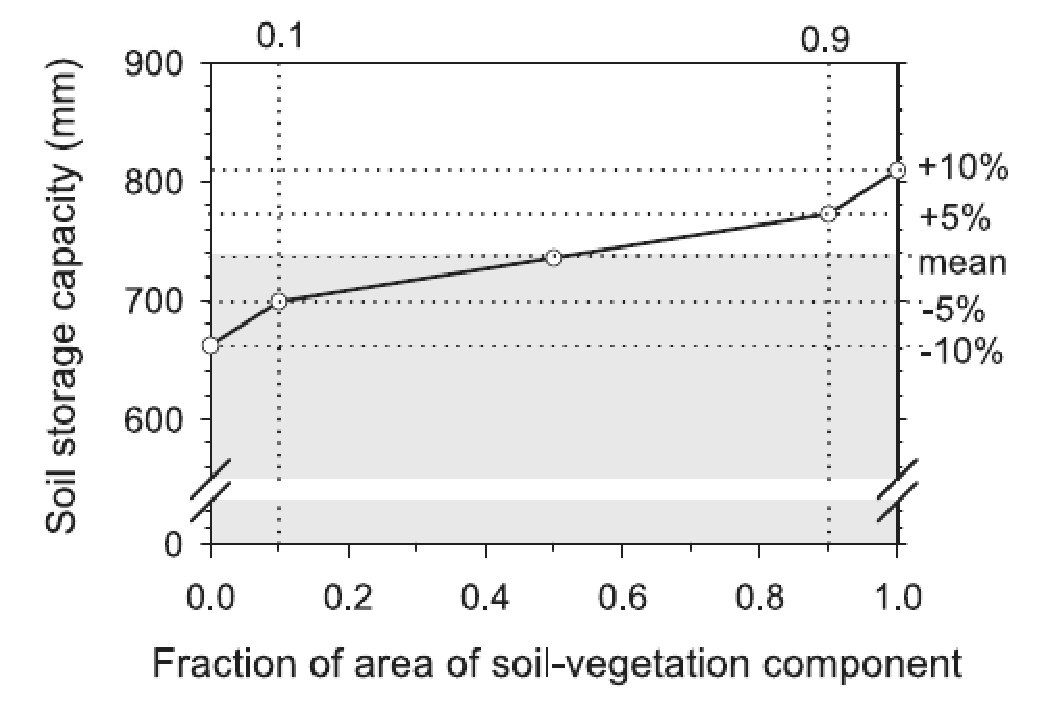
\includegraphics[width=\columnwidth]{\figdir/f_saturation.eps}
  \caption[Example of saturated fraction of a soil unit.]{Example for the computation of saturated fraction of a soil unit from actual water content as given by \eqnref{eq:f_sat}. Graphic copied from \citet{Guentner2002}. \textbf{Units shown deviate from \eqnref{eq:f_sat}!} \label{fig:f_sat}}
\end{figure}

When using function \verb!f_saturation! saturation excess flow can be determined by multiplying incoming surface water flux with the saturated areal fraction of the soil. The remaining part can be given to the infiltration routine. If \verb!f_saturation! is not used saturation excess surface runoff occurs only when the soil is completely saturated (you should check that before calling \verb!infiltration! in order to be able to deviate the two types of surface runoff).


\subsubsection{Subsurface runoff}
Subsurface runoff within the physical based approach can be directly determined from lateral excess runoff (i.e. simply the output of function \verb!latflow!). Further discrimination between a faster (e.g. preferential flow) and slower component is so far not possible.


\subsubsection{Groundwater runoff}
Groundwater runoff (or \emph{baseflow} although in some definitions this also includes slow subsurface runoff) can be deviated from function \verb!percolation!. It is simply the percolation from the deepest soil horizon. To account for travel time through an unsaturated zone below the soil profile a storage routing approach could be applied before adding the percolation output to the groundwater storage.



%%%%%%%%%%%%%%%%%%%%%%%%%%%%%%%%%%%%%%%%%%%%%%%%%%%%%%%%%%%%%%%%%%%%%%%%%%%%%%%%
%%%%%%%%%%%%%%%%%%%%%%%%%%%%%%%%%%%%%%%%%%%%%%%%%%%%%%%%%%%%%%%%%%%%%%%%%%%%%%%%
%%%%%%%%%%%%%%%%%%%%%%%%%%%%%%%%%%%%%%%%%%%%%%%%%%%%%%%%%%%%%%%%%%%%%%%%%%%%%%%%
%%%%%%%%%%%%%%%%%%%%%%%%%%%%%%%%%%%%%%%%%%%%%%%%%%%%%%%%%%%%%%%%%%%%%%%%%%%%%%%%
%%%%%%%%%%%%%%%%%%%%%%%%%%%%%%%%%%%%%%%%%%%%%%%%%%%%%%%%%%%%%%%%%%%%%%%%%%%%%%%%




\section{Contributions and TODOs}
The following work still has to be done or issues need to be resolved:

\begin{itemize}
\item Add more approaches, e.g.
  \begin{itemize}
    \item Better approximation of sorptivity and suction at wetting front \citep{Stewart2013}
    \item Horton: account for soil moisture state and discrete time steps/intermittent rainfall (promising approaches: \citet{Ludwig2010en,Bauer1974,Green1986,Rossman2016})
  \end{itemize}
\item Create separate function to calculate unsaturated hydraulic conductivity and matric potential with several alternatives (so far only \emph{Van Genuchten} considered; could be extended by, e.g., \emph{Brooks and Corey} and/or \emph{Campbell}, \citet{Maidment1993})
\item Include macro pore/preferential flow
\item Include capillary rise
\item Account for ponding of soil profile from lower layers
\item Somehow possible to include the Richards equation? Must be solved numerically, I think each soil layer would have to be somehow subdivided into smaller instances during solving...
\end{itemize}
